\chapter{تغيّرات لا رجعة فيها}\label{ch:g5:irreversible-changes}

نكسر بيضة في مقلاة ساخنة. في ثوانٍ قليلة يصير البياض الرائق السائل
متماسكًا أبيض، ويغلظ الصفار. ارفع المقلاة عن الموقد، ودع البيضة تبرد،
وضعها في الثلاجة: لن تعود بيضة نيئة أبدًا. بعض التغيرات يمكن الرجوع
عنها وبعضها لا يمكن. والتمييز بينهما هو الخطوة الأولى في الكيمياء.

\begin{recall}
الجسم الصلب الذي \omterm{def:g2:mixing-and-dissolving:dissolve}{يذوب} في الماء يبقى موجودًا: فحين يجف الماء يبقى الجسم
الصلب بعده (\cref{ch:g2:mixing-and-dissolving}). \omterm{def:g4:what-a-fire-needs:burning}{والاحتراق} يُنتج مواد
جديدة --- الرماد والدخان وثنائي أكسيد الكربون وبخار الماء --- ويذهب
\omterm{def:g4:what-a-fire-needs:fuel}{الوقود} بلا رجعة (\cref{ch:g4:what-a-fire-needs}).
\end{recall}

\begin{omfigure}
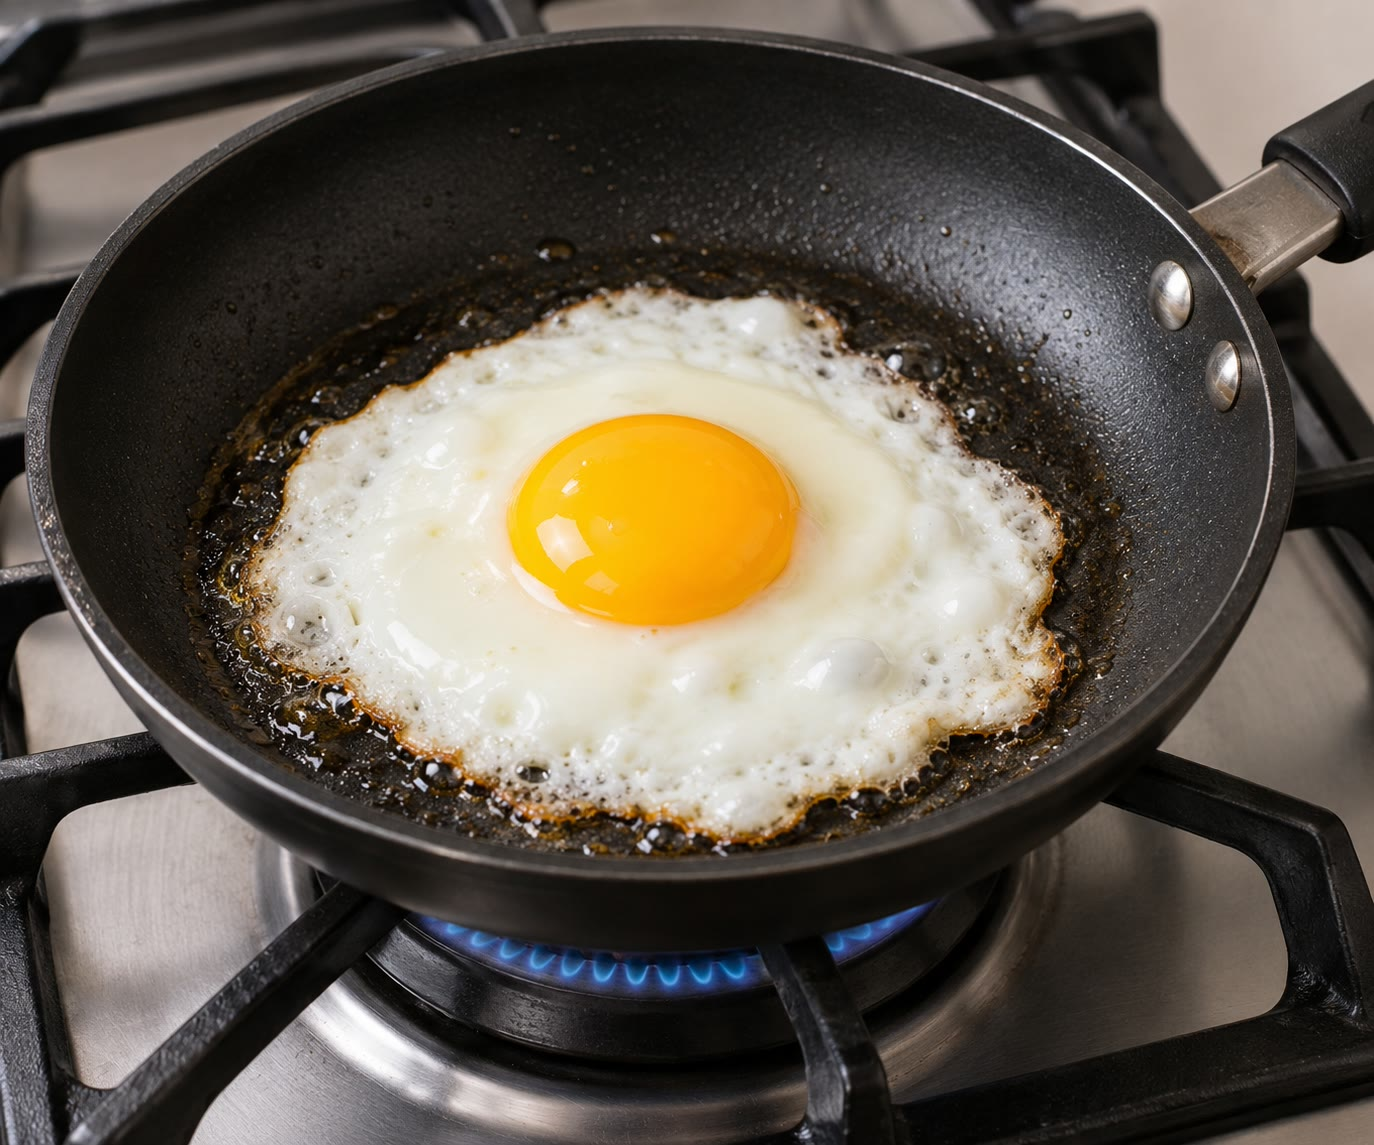
\includegraphics[width=0.55\linewidth]{images/book1/ai/g5-egg-frying.jpg}

{\small بيضة تُقلى: صار البياض الرائق متماسكًا أبيض، بلا
رجعة.}
\end{omfigure}

\section{تغيرات يمكن الرجوع عنها}

\begin{definition}[التغير العكوس]\label{def:g5:irreversible-changes:reversible}
\emph{التغير العكوس}\index{تغير عكوس} تغير يمكن الرجوع عنه، بحيث
نسترجع تمامًا ما بدأنا به.
\end{definition}

\begin{example}[الذوبان والتجفيف]\label{ex:g5:irreversible-changes:dissolve}
السكر الذي نحرّكه في الماء \omterm{def:g2:mixing-and-dissolving:dissolve}{يذوب}. دع الماء يتبخر، فيعود السكر: السكر
نفسه، حلوًا كما كان. \omterm{def:g2:mixing-and-dissolving:dissolve}{فالذوبان} \omterm{def:g5:irreversible-changes:reversible}{تغير عكوس}.
\end{example}

\begin{example}[الجليد والماء]\label{ex:g5:irreversible-changes:ice}
مكعب الجليد على صحن دافئ ينصهر فيصير ماءً؛ ضع الماء في المجمّد فيعود
جليدًا. فالانصهار والتجمد تغيران عكوسان. (أما لماذا ينصهر الماء ويتجمد
فيرويه كتاب الفيزياء.)
\end{example}

\begin{example}[الخلط]\label{ex:g5:irreversible-changes:mix}
الرمل المخلوط بالحصى يمكن أن يُفصل من جديد \omterm{def:g3:separating-mixtures:sieve}{بالغربلة}؛ والماء الموحل يمكن
أن يُرشَّح. \omterm{def:g2:mixing-and-dissolving:mix}{فالخلط} \omterm{def:g5:irreversible-changes:reversible}{تغير عكوس}: لا يُصنع فيه شيء جديد، ويمكن فصل
الأجزاء (\cref{ch:g3:separating-mixtures}).
\end{example}

\section{تغيرات لا يمكن الرجوع عنها}

\begin{definition}[التغير غير العكوس والتغير الكيميائي]\label{def:g5:irreversible-changes:chemical-change}
\emph{التغير غير العكوس}\index{تغير غير عكوس} تغير لا يمكن الرجوع
عنه ببساطة. ومعظم هذه التغيرات تظهر فيها مواد جديدة لم تكن موجودة في
البداية: ويسمى مثل هذا التغير \emph{تغيرًا كيميائيًا}\index{تغير كيميائي}.
\end{definition}

\begin{example}[ستة تغيرات كيميائية]\label{ex:g5:irreversible-changes:six}
\begin{itemize}
  \item \textbf{طهو البيضة}: يصير البياض السائل الشفاف متماسكًا
        أبيض.
  \item \textbf{خَبز الكعكة}: يصير الخليط السائل كعكة إسفنجية،
        بنية من الخارج، ولها رائحة جديدة.
  \item \textbf{\omterm{def:g4:what-a-fire-needs:burning}{الاحتراق}}: يصير الخشب رمادًا ودخانًا وثنائي أكسيد كربون
        وبخار ماء.
  \item \textbf{الصدأ}: الحديد اللامع الذي يُترك تحت المطر يتغطى بمادة
        برتقالية بنية متقشرة هي الصدأ.
  \item \textbf{تحمّض الحليب}: إذا نُسي الحليب أيامًا غلظ، وتكوّنت فيه
        كتل، وصارت رائحته حامضة.
  \item \textbf{اسمرار التفاحة المقطوعة}: يصير لبّها الشاحب بنيًا في
        \omterm{def:g4:air-a-mixture-of-gases:air}{الهواء} في أقل من ساعة.
\end{itemize}
في كل حالة صُنع شيء جديد، ولا توجد طريقة بسيطة لاسترجاع ما بدأنا
به.
\end{example}

\begin{omfigure}
\begin{minipage}[t]{0.48\linewidth}\centering
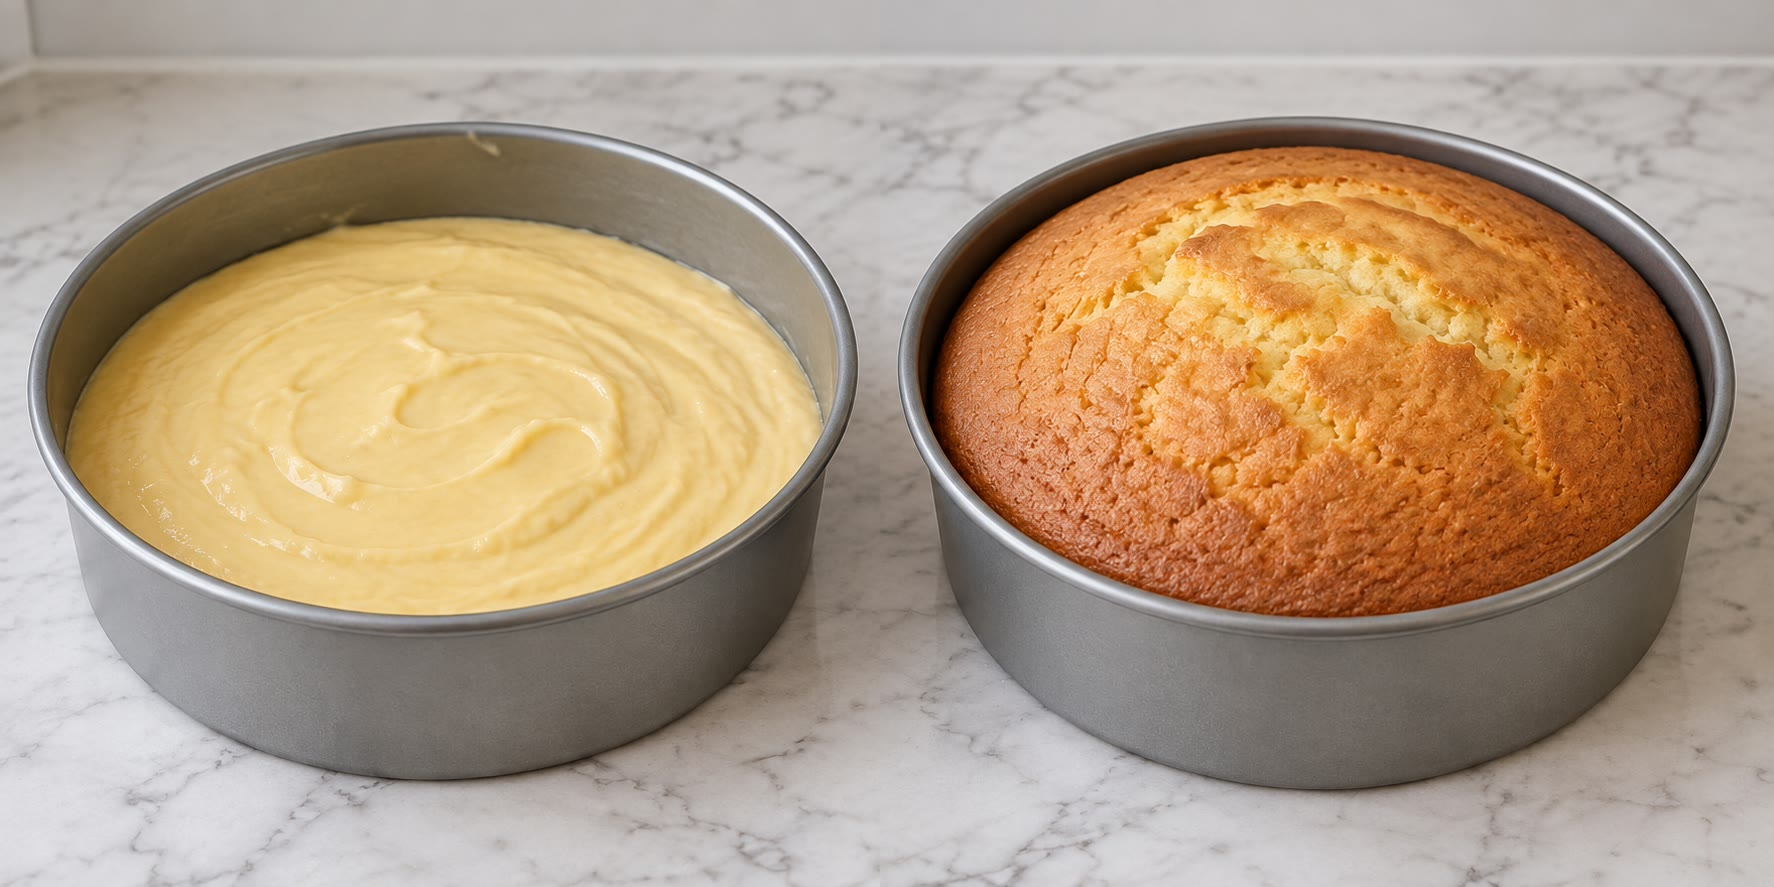
\includegraphics[width=\linewidth,height=4.6cm,keepaspectratio]{images/book1/ai/g5-cake-before-after.jpg}

{\small الخليط قبلُ والكعكة بعدُ: الخَبز لا يمكن الرجوع عنه.}
\end{minipage}\hfill
\begin{minipage}[t]{0.48\linewidth}\centering
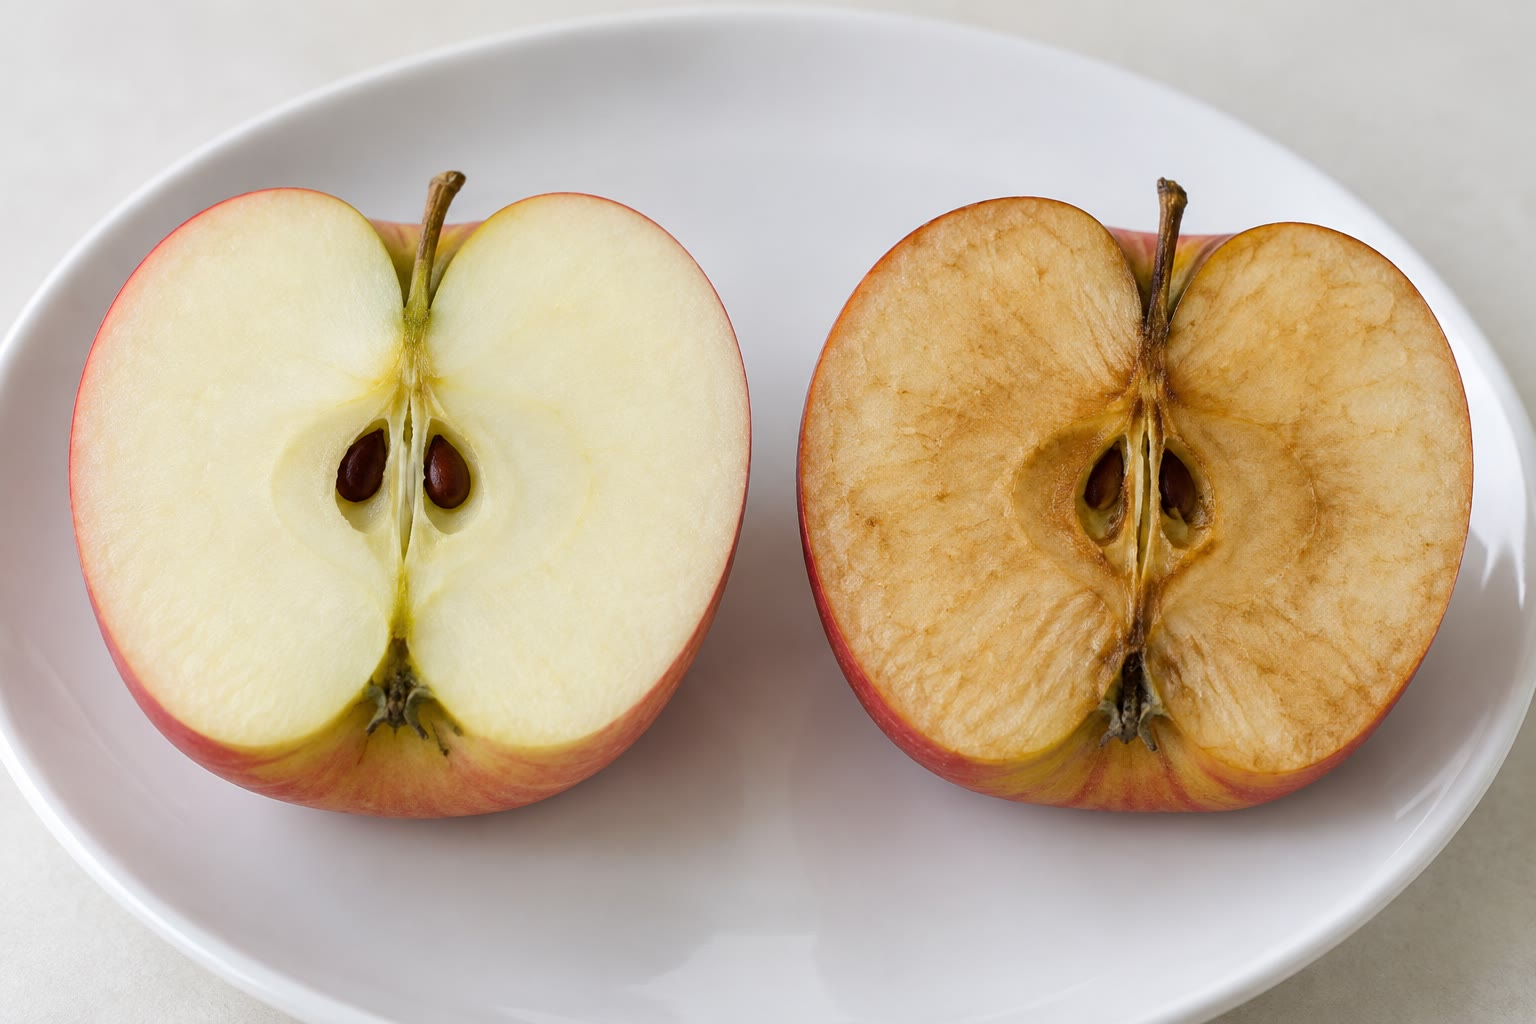
\includegraphics[width=\linewidth,height=4.6cm,keepaspectratio]{images/book1/ai/g5-apple-browning.jpg}

{\small نصف طازج ونصف تُرك ساعة في \omterm{def:g4:air-a-mixture-of-gases:air}{الهواء}.}
\end{minipage}
\end{omfigure}

\begin{omfigure}
\begin{tikzpicture}[font=\small]
  \node[font=\small\bfseries, omDef] at (2.7,4.6) {يمكن الرجوع عنها};
  \node[font=\small\bfseries, omProp] at (9.6,4.6) {لا يمكن الرجوع عنها};
  \draw[black!30] (6.1,4.9) -- (6.1,-0.3);
  % reversible pairs
  \foreach \y/\a/\b in {3.6/{سكر + ماء}/{ماء محلّى}, 2.0/{جليد}/{ماء سائل},
                        0.4/{رمل + حصى}/{خليط}} {
    \node[draw=omDef, fill=omDef!6, rounded corners=2pt, minimum width=2.3cm,
      minimum height=0.8cm] at (0.9,\y) {\a};
    \node[draw=omDef, fill=omDef!6, rounded corners=2pt, minimum width=2.3cm,
      minimum height=0.8cm] at (4.6,\y) {\b};
    \draw[->, thick, omDef] (2.3,\y+0.12) -- (3.25,\y+0.12);
    \draw[<-, thick, omDef] (2.3,\y-0.12) -- (3.25,\y-0.12);
  }
  % irreversible ones
  \foreach \y/\a/\b in {3.6/{بيضة نيئة}/{بيضة مطهوة}, 2.0/{خشب}/{رماد، دخان، غازات},
                        0.4/{حديد}/{صدأ}} {
    \node[draw=omProp, fill=omProp!6, rounded corners=2pt, minimum width=2.0cm,
      minimum height=0.8cm] at (7.6,\y) {\a};
    \node[draw=omProp, fill=omProp!6, rounded corners=2pt, minimum width=2.9cm,
      minimum height=0.8cm] at (11.5,\y) {\b};
    \draw[->, thick, omProp] (8.8,\y) -- (9.85,\y);
  }
\end{tikzpicture}

{\small يسارًا: تغيرات عكوسة، والسهم المزدوج يعني أنها تسير في
الاتجاهين. يمينًا: تغيرات كيميائية، في اتجاه واحد فقط.}
\end{omfigure}

\section{علامات تدل على ظهور مادة جديدة}

\begin{method}[أهو تغير كيميائي؟ ابحث عن العلامات]\label{met:g5:irreversible-changes:clues}
كثيرًا ما تكشف عن المادة الجديدة إحدى هذه العلامات:
\begin{enumerate}
  \item \textbf{لون} جديد (اللون البني لشريحة خبز محمّصة)؛
  \item \textbf{فقاعات} غاز تظهر في سائل دون أي تسخين (الخل يُصب على
        صودا الخبز)؛
  \item \textbf{رائحة} جديدة (الحليب الحامض، الخبز المحمّص المحترق)؛
  \item \textbf{حرارة أو ضوء} ينطلقان (شمعة مشتعلة)؛
  \item \textbf{جسم صلب يظهر} في سائل رائق، أو كتل تتكوّن
        (تخثر الحليب).
\end{enumerate}
وعلامة واحدة وحدها قد تضلل: فالماء الذي يغلي تظهر فيه فقاعات، لكن لا
يُصنع شيء جديد --- فالفقاعات بخار ماء، ويعود الماء حين يبرد البخار.
فابحث عن عدة علامات، واسأل: هل يمكن الرجوع عنه؟
\end{method}

\begin{omfigure}
\begin{tikzpicture}[font=\small]
  \foreach \k/\t in {0/{لون جديد}, 1/{فقاعات غاز}, 2/{رائحة جديدة},
                     3/{حرارة أو ضوء}, 4/{ظهور جسم صلب}} {
    \begin{scope}[xshift=\k*3.2cm]
      \draw[omProp, line width=0.8pt, fill=omProp!5] (0,0) circle (1.0);
      \node[anchor=north, align=center] at (0,-1.15) {\t};
    \end{scope}
  }
  % 1: colour, a slice of toast half brown
  \fill[yellow!20, draw=brown!60] (-0.55,-0.5) rectangle (0.55,0.55);
  \fill[brown!55] (0,-0.5) rectangle (0.55,0.55);
  % 2: bubbles in a beaker
  \begin{scope}[xshift=3.2cm]
    \pic[transform shape, scale=0.45] at (0,-0.55) {beaker={0.7}{omWater!80}};
    \foreach \x/\y in {-0.15/-0.2,0.1/0.05,-0.05/0.25,0.18/-0.35,-0.2/0.15}
      \draw[black!55] (\x,\y) circle (0.05);
  \end{scope}
  % 3: smell, wavy lines
  \begin{scope}[xshift=6.4cm]
    \foreach \x in {-0.35,0,0.35} \draw[black!55, line width=0.8pt, decorate,
      decoration={snake, amplitude=1.5pt, segment length=6pt}] (\x,-0.6) -- (\x,0.6);
  \end{scope}
  % 4: a flame
  \begin{scope}[xshift=9.6cm]
    \fill[orange!80] (0,-0.6) .. controls (-0.45,-0.05) and (-0.15,0.35) .. (0,0.7)
      .. controls (0.15,0.35) and (0.45,-0.05) .. (0,-0.6);
    \fill[yellow!80] (0,-0.45) .. controls (-0.2,-0.1) and (-0.08,0.15) .. (0,0.3)
      .. controls (0.08,0.15) and (0.2,-0.1) .. (0,-0.45);
  \end{scope}
  % 5: solid settling in a test tube
  \begin{scope}[xshift=12.8cm]
    \pic[transform shape, scale=0.4] at (0,-0.65) {testtube={0.75}{omWater!80}};
    \fill[white, draw=black!40] (-0.08,-0.62) rectangle (0.08,-0.5);
    \foreach \x/\y in {-0.04/-0.3,0.04/-0.1,0/0.1} \fill[black!35] (\x,\y) circle (0.03);
  \end{scope}
\end{tikzpicture}

{\small خمس علامات تدل على أن \omterm{def:g5:irreversible-changes:chemical-change}{تغيرًا كيميائيًا} ربما حدث.}
\end{omfigure}

\begin{inthelab}[الخل على صودا الخبز]
يضع المعلم ملعقة من صودا الخبز، وهي مسحوق أبيض، في قاع كأس، ثم يصب
فيها قليلًا من الخل. فيفور الخليط ويرغي في الحال: ينطلق غاز، وهذه علامة
على \omterm{def:g5:irreversible-changes:chemical-change}{تغير كيميائي}. وحين يتوقف الفوران تكون صودا الخبز قد اختفت، ولا يمكن
استرجاعها بالتجفيف.
\end{inthelab}

\begin{omfigure}
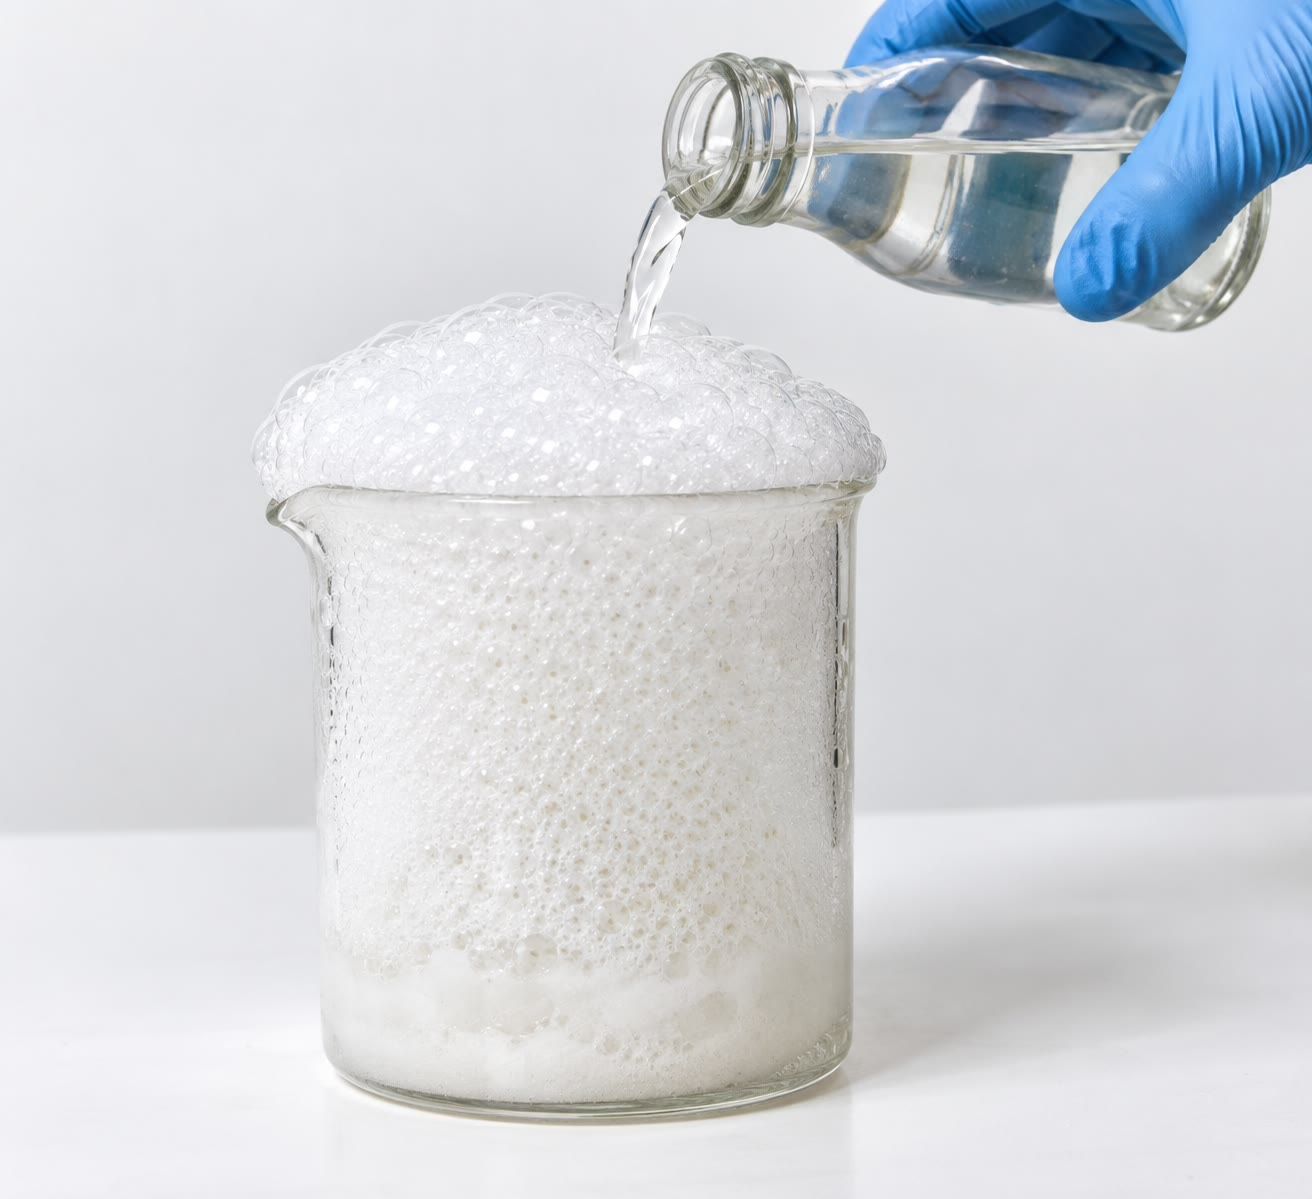
\includegraphics[width=0.5\linewidth]{images/book1/ai/g5-baking-soda-lab.jpg}

{\small الخل على صودا الخبز: ينطلق غاز.}
\end{omfigure}

\section{تغيرات نافعة وتغيرات ضارة}

\begin{proposition}[التغيرات الكيميائية من حولنا]\label{prop:g5:irreversible-changes:around}
كثير من التغيرات الكيميائية نافع: طهو الطعام، وخَبز الخبز، وحرق الغاز
لتدفئة البيت، وتصلّب الجص أو الإسمنت. وبعضها الآخر يُحدث ضررًا: صدأ
الحديد، وفساد الطعام، وتعفن الخشب. لا نستطيع الرجوع عنها، لكننا
نستطيع إبطاءها:
\begin{itemize}
  \item يحفظ الطعام مدة أطول في برد الثلاجة؛
  \item الطلاء أو طبقة رقيقة من الزيت يُبعدان \omterm{def:g4:air-a-mixture-of-gases:air}{الهواء} والماء عن الحديد؛
  \item التفاحة المقطوعة المرشوشة بعصير الليمون تسمرّ ببطء أكبر.
\end{itemize}
\end{proposition}

\begin{omfigure}
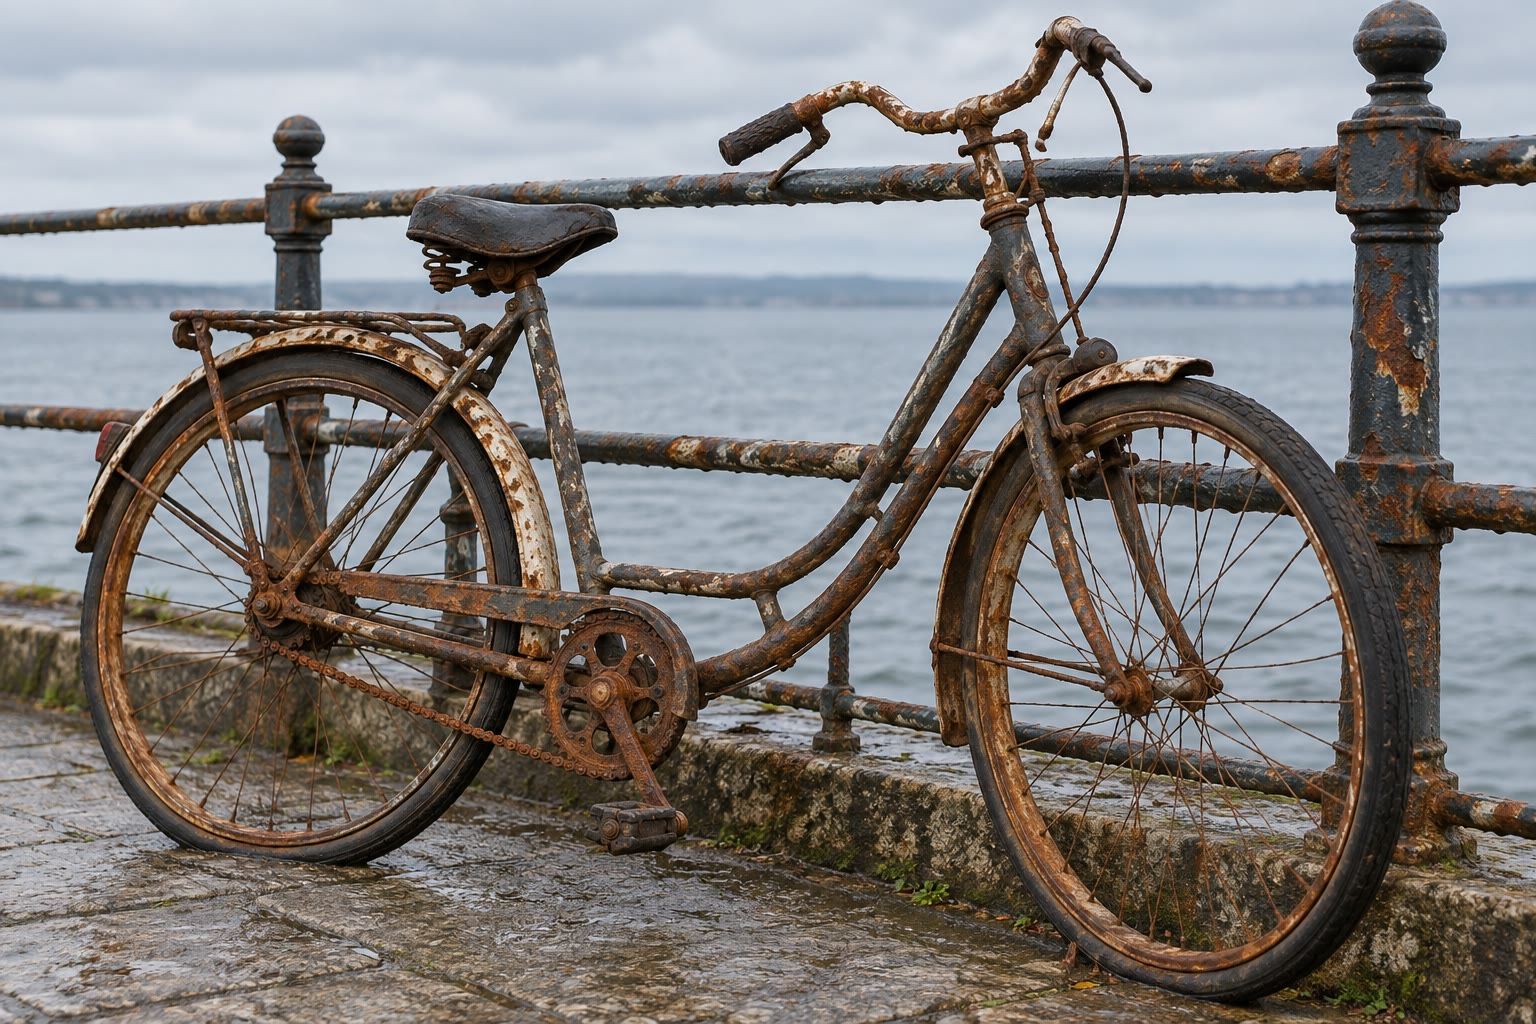
\includegraphics[width=0.55\linewidth]{images/book1/ai/g5-rusty-bicycle.jpg}

{\small دراجة تُركت تحت المطر سنوات: صدئ الحديد.}
\end{omfigure}

\begin{remark}[الرجوع ممكن، لكن ليس ببساطة]\label{rem:g5:irreversible-changes:not-simply}
«لا يمكن الرجوع عنه» تعني أنه لا توجد طريق بسيطة للعودة، مثل التبريد
أو التجفيف. فقد يستطيع الكيميائيون أحيانًا أن يعيدوا الصدأ حديدًا، لكن
بفرن ومواد جديدة فقط: وذلك \omterm{def:g5:irreversible-changes:chemical-change}{تغير كيميائي} آخر، لا رجوع عن
التغير الأول.
\end{remark}

\section{تمارين}

\begin{exercise}[$\star$]\label{exo:g5:irreversible-changes:1}
قل عن كل تغير هل يمكن الرجوع عنه: انصهار الشوكولاتة، \omterm{def:g4:what-a-fire-needs:burning}{واحتراق} عود
ثقاب، \omterm{def:g2:mixing-and-dissolving:dissolve}{وذوبان} الملح في الماء، وتحميص الخبز.
\end{exercise}

\begin{exercise}[$\star$]\label{exo:g5:irreversible-changes:2}
ما \omterm{def:g5:irreversible-changes:chemical-change}{التغير الكيميائي}؟ أعطِ مثالين من المطبخ.
\end{exercise}

\begin{exercise}[$\star$]\label{exo:g5:irreversible-changes:3}
يُذاب ملح في الماء. كيف نسترجع الملح؟ وهل \omterm{def:g2:mixing-and-dissolving:dissolve}{الذوبان} \omterm{def:g5:irreversible-changes:reversible}{تغير
عكوس}؟
\end{exercise}

\begin{exercise}[$\star$]\label{exo:g5:irreversible-changes:4}
أي علامة من علامات \omterm{def:g5:irreversible-changes:chemical-change}{التغير الكيميائي} تلاحظها حين يتحمض الحليب؟
أعطِ علامتين.
\end{exercise}

\begin{exercise}[$\star$]\label{exo:g5:irreversible-changes:5}
انظر إلى الشكل الذي فيه عمودان. أي التغيرات لها سهم مزدوج؟ وماذا يعني
السهم المزدوج؟
\end{exercise}

\begin{exercise}[$\star$]\label{exo:g5:irreversible-changes:6}
لماذا تُزيَّت سلسلة الدراجة؟ وأي \omterm{def:g5:irreversible-changes:chemical-change}{تغير كيميائي} يبطئه
الزيت؟
\end{exercise}

\begin{exercise}[$\star$]\label{exo:g5:irreversible-changes:7}
حين يُصب الخل على صودا الخبز يفور. أي علامة هذه؟
\end{exercise}

\begin{exercise}[$\star$]\label{exo:g5:irreversible-changes:8}
سمِّ \omterm{def:g5:irreversible-changes:chemical-change}{تغيرًا كيميائيًا} نافعًا \omterm{def:g5:irreversible-changes:chemical-change}{وتغيرًا كيميائيًا} ضارًا.
\end{exercise}

\begin{exercise}[$\star$]\label{exo:g5:irreversible-changes:9}
لماذا نحفظ الحليب في الثلاجة؟
\end{exercise}

\begin{exercise}[$\star\star$]\label{exo:g5:irreversible-changes:10}
تظهر فقاعات في الماء حين يغلي. هل الغليان \omterm{def:g5:irreversible-changes:chemical-change}{تغير كيميائي}؟ اشرح لماذا لا
تكفي علامة واحدة.
\end{exercise}

\begin{exercise}[$\star\star$]\label{exo:g5:irreversible-changes:11}
يقول توم: «حين تشتعل الشمعة فإن الشمع ينصهر ويذهب فقط، مثل الجليد.»
استعمل علامتين لتشرح لماذا يُعدّ \omterm{def:g4:what-a-fire-needs:burning}{احتراق} الشمعة \omterm{def:g5:irreversible-changes:chemical-change}{تغيرًا كيميائيًا}، وليس
انصهارًا فقط.
\end{exercise}
